\documentclass[]{article}
\usepackage{lmodern}
\usepackage{amssymb,amsmath}
\usepackage{ifxetex,ifluatex}
\usepackage{fixltx2e} % provides \textsubscript
\ifnum 0\ifxetex 1\fi\ifluatex 1\fi=0 % if pdftex
  \usepackage[T1]{fontenc}
  \usepackage[utf8]{inputenc}
\else % if luatex or xelatex
  \ifxetex
    \usepackage{mathspec}
  \else
    \usepackage{fontspec}
  \fi
  \defaultfontfeatures{Ligatures=TeX,Scale=MatchLowercase}
\fi
% use upquote if available, for straight quotes in verbatim environments
\IfFileExists{upquote.sty}{\usepackage{upquote}}{}
% use microtype if available
\IfFileExists{microtype.sty}{%
\usepackage{microtype}
\UseMicrotypeSet[protrusion]{basicmath} % disable protrusion for tt fonts
}{}
\usepackage[margin=1in]{geometry}
\usepackage{hyperref}
\hypersetup{unicode=true,
            pdftitle={Untitled},
            pdfauthor={Daniel Hsiao},
            pdfborder={0 0 0},
            breaklinks=true}
\urlstyle{same}  % don't use monospace font for urls
\usepackage{graphicx,grffile}
\makeatletter
\def\maxwidth{\ifdim\Gin@nat@width>\linewidth\linewidth\else\Gin@nat@width\fi}
\def\maxheight{\ifdim\Gin@nat@height>\textheight\textheight\else\Gin@nat@height\fi}
\makeatother
% Scale images if necessary, so that they will not overflow the page
% margins by default, and it is still possible to overwrite the defaults
% using explicit options in \includegraphics[width, height, ...]{}
\setkeys{Gin}{width=\maxwidth,height=\maxheight,keepaspectratio}
\IfFileExists{parskip.sty}{%
\usepackage{parskip}
}{% else
\setlength{\parindent}{0pt}
\setlength{\parskip}{6pt plus 2pt minus 1pt}
}
\setlength{\emergencystretch}{3em}  % prevent overfull lines
\providecommand{\tightlist}{%
  \setlength{\itemsep}{0pt}\setlength{\parskip}{0pt}}
\setcounter{secnumdepth}{5}
% Redefines (sub)paragraphs to behave more like sections
\ifx\paragraph\undefined\else
\let\oldparagraph\paragraph
\renewcommand{\paragraph}[1]{\oldparagraph{#1}\mbox{}}
\fi
\ifx\subparagraph\undefined\else
\let\oldsubparagraph\subparagraph
\renewcommand{\subparagraph}[1]{\oldsubparagraph{#1}\mbox{}}
\fi

%%% Use protect on footnotes to avoid problems with footnotes in titles
\let\rmarkdownfootnote\footnote%
\def\footnote{\protect\rmarkdownfootnote}

%%% Change title format to be more compact
\usepackage{titling}

% Create subtitle command for use in maketitle
\newcommand{\subtitle}[1]{
  \posttitle{
    \begin{center}\large#1\end{center}
    }
}

\setlength{\droptitle}{-2em}
  \title{Untitled}
  \pretitle{\vspace{\droptitle}\centering\huge}
  \posttitle{\par}
  \author{Daniel Hsiao}
  \preauthor{\centering\large\emph}
  \postauthor{\par}
  \predate{\centering\large\emph}
  \postdate{\par}
  \date{November 12, 2018}


\begin{document}
\maketitle

{
\setcounter{tocdepth}{3}
\tableofcontents
}
\newpage

\hypertarget{methodology}{%
\section{Methodology}\label{methodology}}

\hypertarget{threshold-truncation}{%
\section{Threshold Truncation}\label{threshold-truncation}}

\hypertarget{standard-approach}{%
\subsection{Standard Approach}\label{standard-approach}}

\hypertarget{truncation-approach}{%
\subsection{Truncation Approach}\label{truncation-approach}}

\hypertarget{bias-correction}{%
\subsection{Bias Correction}\label{bias-correction}}

\hypertarget{survey-of-professional-forecasters-spf}{%
\section{Survey of Professional Forecasters
(SPF)}\label{survey-of-professional-forecasters-spf}}

To illustrate the empirical results, we use the data from ECB
\emph{(footnote link to data)} in this paper. The data, SPF, is a
quarterly survey initiated by ECB, with the aim to obtain future
estimates on inflation (HICP), RGDP and unemployment rate (UNEM) from
the private sector. Every quarter, a gourp of professional forecasters
from financial and non-financial instutition, such as economic research
institutions, respond to the survey with the idea on the future
economic. Starting 1999, SPF is the longest survey of macroeconomic
expectation in the euro area. Until the date of this report, there are
75 quarters of observation available, with 1999 Q4 as the first
forecasted value, and 2018 Q2 as the last observed true macroeconomic
indice.

The set up of the survey consist of multiple magnitudes of questions,
ranging from different horizon to different distribution. The
forecaststers are asked to provide their point forecast and the
probability of a certain scenario to happen. This enables ECB to do
quantitative assessment on the consensus of the market, like the
distribution statistics and standard deviations. For this paper, we take
the 2 most answered time periods, which is 1 year ahead and 2 year ahead
as our data set for all HICP, RGDP, and UNEM.

To compare the forecasts with the actual macroeconomics, we obtain the
true value from ECB data base \emph{(footnote link to data)}. The data
cannot be observed from the economic in 100\% accuracy within the first
time frame, and exihibits changes to the initial estimates after
revision. We use the final estimate of the macroeconomics where
possible. This is due to the fact that the original forecast is not the
real target to be forecasts.

\begin{figure}[!h]
\centering
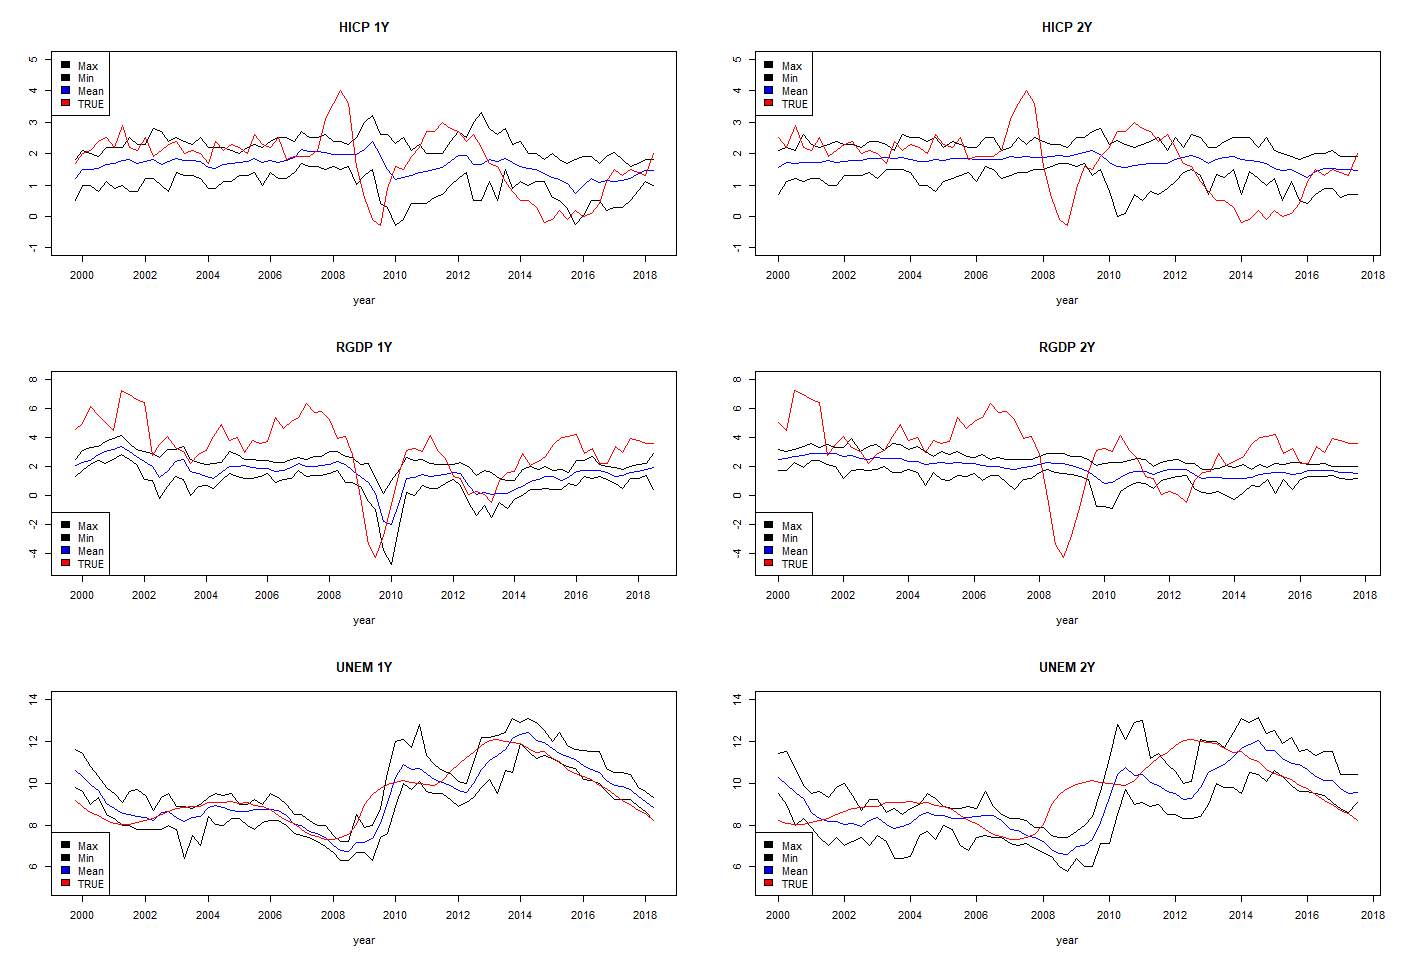
\includegraphics[width=16cm, height=26cm]{./Output/Images/SPF.png}
\caption{Survey of Professional Forecasters data illustration}\label{SPF data illustration}
\end{figure}

In figure \ref{SPF data illustration} and table \emph{(label table)} we
show the plots and the statistics of the forecasts, along side with the
true value in the macroeconomics. To avoid too many lines on the figure
by plotting all forecasts, we plot only the minimum, mean, and maximum
from the forecasts. We see that there exist a high consistency across
all forecasts, with 2 year ahead stronger than 1 year. The consistency
in the forecast is lower in UNEM than the other two. Furthermore, many
true values lies outside of the forecast range, with RGDP the worse of
all three.

\textbf{add more explanation}

\hypertarget{empirical-results}{%
\section{Empirical Results}\label{empirical-results}}


\end{document}
